\chapter{Metodologia}

\section{Simulação}

% Falar do octave

% A simulação do sistema proposto foi construída utilizando o \textit{software} GNU Octave e suas bibliot


A construção da simulação partiu de uma abordagem físico-matemática, definindo o sinal \ac{w} como uma função de onda relativa ao tempo e ao espaço, analisando seus valores incidindo em cada antena \ac{Ak} e comparando as defasagens \ac{DeltaPhi} entre os diferentes pares de antenas.
Para simplificar a construção da simulação, foram utilizadas funções paramétricas, descritas na presente seção.

\subsection{Parâmetros envolvidos}

Com o objetivo de garantir a coerência entre as partes da simulação, vários parâmetros foram utilizados, definindo detalhes em relação às operações matemáticas e às formas de registro dos valores calculados.
Estes parâmetros são divididos entre os que recebem valores numéricos, booleanos ou matrizes numéricas.

Os parâmetros numéricos são:
\begin{itemize}
	\item \lstinline|amp_w|, amplitude desejada para o sinal;
	\item \lstinline|ang_w|, direção do emissor do sinal, equivalente ao ângulo \ac{thetaAoA} de chegada do sinal em relacao à malha de antenas;
	\item \lstinline|angle_Z_A_x_B|, ângulo relativo \ac{betak} para par de antenas;
	\item \lstinline|d|, distância \ac{d} entre par de antenas da malha;
	\item \lstinline|choose_angle|, ângulo \ac{thetaAoA} calculado pelo sistema;
	\item \lstinline|interval|, indica os limites para a geração de imagem da simulação;
	\item \lstinline|lambda_w|, comprimento de onda \ac{lambda};
	\item \lstinline|N_antenas|, quantidade \ac{Nant} de antenas da malha;
	\item \lstinline|omega_w|, frêquencia angular \ac{omega};
	\item \lstinline|phase_w|, fase $\phi$ do sinal no emissor;
	\item \lstinline|Rho|, raio \ac{rho} do polígono que dispõe as antenas na malha;
	\item \lstinline|r_w|, distância que o emissor de sinal está da coordenada $(0,~0)$ do sistema;
	\item \lstinline|range_step|, largura em graus do passo na simulação.
	\item \lstinline|resolution|, relativo à quantidade de pontos utilizados na aproximação numérica do cálculo de correlação;
	\item \lstinline|SNR|, valor da \ac{SNR} linear;
	\item \lstinline|SNR_dB|, valor da \ac{SNR} em \si{\decibel};
	\item \lstinline|t_w|, tempo $t$ associado ao instante de aferição do sinal;
	\item \lstinline|x_w| ou \lstinline|y_w|, coordenada \ac{xk} ou \ac{yk} da antena \ac{Ak} em relação ao sistema;
	\item \lstinline|Z_antenna|, \lstinline|Z_antenna_A| ou \lstinline|Z_antenna_B|, valor complexo, coordenada de antena;
	\item \lstinline|Z_phase_A| ou \lstinline|Z_phase_B|, valor complexo, fase \ac{Phik} de antena;
\end{itemize}

Os parâmetros booleanos são:
\begin{itemize}
	\item \lstinline|ATT|, indica se o sinal contará com atenuação por distância;
	\item \lstinline|C|, indica a utilização de componente cossenoidal na construção do sinal;
	\item \lstinline|CHG_PHI|, indica se a fase geral do sinal deve mudar ao longo da simulação;
	\item \lstinline|CHG_R|, indica se a distância do emissor do sinal deverá mudar ao longo da simulação;
	\item \lstinline|CHG_THETA|, indica se o ângulo de origem do sinal deverá mudar ao longo da simulação;
	\item \lstinline|NOISE|, indica se o sinal contará com ruído;
	\item \lstinline|S|, indica a utilização de componente senoidal na construção do sinal;
	\item \lstinline|S_DAT|, indica se os pontos gerados pela simulação deverão ser salvos;
	\item \lstinline|S_GIF|, indica se a imagem gerada pela simulação deverá ser salva;
\end{itemize}

Os parâmetros de matrizes numéricas são:
\begin{itemize}
	\item \lstinline|ant_array|, coordenadas das antenas da malha;
	\item \lstinline|delta_A_x_B_array|, contendo o ângulo \ac{thetak} calculado por $\ac{alphak} + \ac{betak}$ aferido para cada par de antenas da malha;
	\item \lstinline|delta_B_x_A_array|, contendo o ângulo \ac{thetak} calculado por $\ac{alphak} - \ac{betak}$ aferido para cada par de antenas da malha;
	\item \lstinline|Z_phase_array|, matriz de valores numéricos complexos, contendo o sinal complexo aferido para cada antena da malha;
	\item \lstinline|z_plot|, estado corrente do sinal no espaço, utilizado na geração de imagem da simulação;
	\item \lstinline|Z_x_array|, valores complexos, contendo a defasagem \ac{DeltaPhi} aferido para cada par de antenas na malha;
\end{itemize}







% Estes parâmetros são:
% \begin{itemize}
% 	\item \lstinline|amp_w|, valor numérico, amplitude desejada para o sinal;
% 	\item \lstinline|ang_w|, valor numérico, direção do emissor do sinal, equivalente ao ângulo \ac{thetaAoA} de chegada do sinal em relacao à malha de antenas;
% 	\item \lstinline|angle_Z_A_x_B|, valor numérico, ângulo relativo \ac{betak} para par de antenas;
% 	\item \lstinline|ant_array|, matriz de valores numéricos, coordenadas das antenas da malha;
% 	\item \lstinline|d|, valor numérico, distância \ac{d} entre par de antenas da malha;
% 	\item \lstinline|delta_A_x_B_array|, matriz de valores numéricos, contendo o ângulo \ac{thetak} calculado por $\ac{alphak} + \ac{betak}$ aferido para cada par de antenas da malha;
% 	\item \lstinline|delta_B_x_A_array|, matriz de valores numéricos, contendo o ângulo \ac{thetak} calculado por $\ac{alphak} - \ac{betak}$ aferido para cada par de antenas da malha;
% 	\item \lstinline|choose_angle|, valor numérico, ângulo \ac{thetaAoA} calculado pelo sistema;
% 	\item \lstinline|interval|, valor numérico, indica os limites para a geração de imagem da simulação;
% 	\item \lstinline|lambda_w|, valor numérico, comprimento de onda \ac{lambda};
% 	\item \lstinline|omega_w|, valor numérico, frêquencia angular \ac{omega};
% 	\item \lstinline|phase_w|, valor numérico, fase $\phi$ do sinal no emissor;
% 	\item \lstinline|r_w|, valor numérico, distância que o emissor de sinal está da coordenada $(0, 0)$ do sistema;
% 	\item \lstinline|range_step|, valor numérico, largura em graus do passo na simulação.
% 	\item \lstinline|resolution|, valor numérico, relativo à quantidade de pontos utilizados na aproximação numérica do cálculo de correlação;
% 	\item \lstinline|t_w|, valor numérico, tempo $t$ associado ao instante de aferição do sinal;
% 	\item \lstinline|x_w| ou \lstinline|y_w|, valor numérico, coordenada \ac{xk} ou \ac{yk} da antena \ac{Ak} em relação ao sistema;
% 	% \item \lstinline|x_w|, valor numérico, coordenada \ac{xk} da antena em questão em relação ao sistema;
% 	% \item \lstinline|y_w|, valor numérico, coordenada \ac{yk} da antena em questão em relação ao sistema;
% 	\item \lstinline|z_plot|, matriz de valores numéricos, estado corrente do sinal no espaço, utilizado na geração de imagem da simulação;

% 	\item \lstinline|ATT|, valor binário, indica se o sinal contará com atenuação por distância;
% 	\item \lstinline|CHG_PHI|, valor binário, indica se a fase geral do sinal deve mudar ao longo da simulação;
% 	\item \lstinline|CHG_R|, valor binário, indica se a distância do emissor do sinal deverá mudar ao longo da simulação;
% 	\item \lstinline|CHG_THETA|, valor binário, indica se o ângulo de origem do sinal deverá mudar ao longo da simulação;
% 	\item \lstinline|C|, valor binário, indica a utilização de componente cossenoidal na construção do sinal;
% 	\item \lstinline|N_antenas|, valor numérico, quantidade \ac{Nant} de antenas da malha;
% 	\item \lstinline|NOISE|, valor binário, indica se o sinal contará com ruído;
% 	\item \lstinline|Rho|, valor numérico, raio \ac{rho} do polígono que dispõe as antenas na malha;
% 	\item \lstinline|S_GIF|, valor binário, indica se a imagem gerada pela simulação deverá ser salva;
% 	\item \lstinline|S_DAT|, valor binário, indica se os pontos gerados pela simulação deverão ser salvos;
% 	\item \lstinline|S|, valor binário, indica a utilização de componente senoidal na construção do sinal;
% 	\item \lstinline|SNR_dB|, valor numérico, valor da \ac{SNR} em \si{\decibel};
% 	\item \lstinline|SNR|, valor numérico, valor da \ac{SNR} linear;
% 	\item \lstinline|Z_antenna|, \lstinline|Z_antenna_A| ou \lstinline|Z_antenna_B|, valor numérico complexo, coordenada de antena;
% 	% \item \lstinline|Z_antenna_A|, valor numérico complexo, coordenada de antena \ac{Ak};
% 	% \item \lstinline|Z_antenna_B|, valor numérico complexo, coordenada de antena \ac{Ak};
% 	\item \lstinline|Z_phase_array|, matriz de valores numéricos complexos, contendo o sinal complexo aferido para cada antena da malha;
% 	\item \lstinline|Z_phase_A| ou \lstinline|Z_phase_B|, valor numérico complexo, fase \ac{Phik} de antena;
% 	% \item \lstinline|Z_phase_B|, valor numérico complexo, fase \ac{Phik} de antena \ac{Ak};
% 	\item \lstinline|Z_x_array|, matriz de valores numéricos complexos, contendo a defasagem \ac{DeltaPhi} aferido para cada par de antenas na malha;
% \end{itemize}

\subsection{Funções auxiliares}

% argument_r
A primeira função a ser definida é \lstinline|argument_r|, que opera como auxiliar para normalização de argumento para as funções trigonométricas utilizadas nas análises, garantindo coerência em frequência angular e coordenadas espaciais.
Seus argumentos são, respectivamente, \lstinline|x_w|, \lstinline|y_w|, \lstinline|t_w|, \lstinline|ang_w|, \lstinline|r_w|, \lstinline|lambda_w| e \lstinline|omega_w|.
O \autoref{cod:argument_r} apresenta uma versão simplificada da função \lstinline|argument_r| desenvolvida.

\begin{lstfloat}[htbp]
	\centering
	\lstinputlisting[
			basicstyle=\ttfamily\small\setstretch{1},
			label=cod:argument_r,
			caption={Função \lstinline|argument_r|, simplificada.}
		]{../code/argument_r_alt.m}
	\caption*{Fonte: Autor.}
\end{lstfloat}

% Carregar bibliotecas

% ref_sin e ref_cos
Para determinar a fase do sinal \ac{w}, incidente em cada antena \ac{Ak}, calcula-se a correlação deste sinal com sinais de referência seno e cossenos, fornecidos respectivamente pelas funções \lstinline|ref_sin| e \lstinline|ref_cos|.
As duas funções recebem os mesmos argumentos, e estes são, respectivamente, \lstinline|t_w| e \lstinline|omega_w|.
Ambos os casos utilizam a função \lstinline|argument_r| para garantir coerência de frequência com o sinal incidente.
Os Códigos \ref{cod:ref_cos} e \ref{cod:ref_sin} apresentam, respectivamente, versões simplificadas das funções \lstinline|ref_cos| e \lstinline|ref_sin| desenvolvidas.


\begin{lstfloat}[htbp]
	\centering
	\lstinputlisting[
			basicstyle=\ttfamily\small\setstretch{1},
			label=cod:ref_cos,
			caption={Função \lstinline|ref_cos|, simplificada.}
		]{../code/ref_cos_alt.m}
	\caption*{Fonte: Autor.}
\end{lstfloat}

\begin{lstfloat}[htbp]
	\centering
	\lstinputlisting[
			basicstyle=\ttfamily\small\setstretch{1},
			label=cod:ref_sin,
			caption={Função \lstinline|ref_sin|, simplificada.}
		]{../code/ref_sin_alt.m}
	\caption*{Fonte: Autor.}
\end{lstfloat}


% signal_r
A próxima função contruída foi \lstinline|signal_r|, que calcula o valor do sinal \ac{w} numa coordenada $(x,~y)$ e um instante $t$.
Considera-se que o sinal é composto pela soma de seno e cosseno, e que são determinadas a distância e a direção de sua fonte emissora.
Também é possível definir amplitude e fase na origem, além da presença de atenuação e ruído do tipo \ac{AWGN}.
Seus argumentos são, respectivamente, \lstinline|x_w|, \lstinline|y_w|, \lstinline|t_w|, \lstinline|amp_w|, \lstinline|ang_w|, \lstinline|r_w|, \lstinline|phase_w|, \lstinline|lambda_w|, \lstinline|omega_w|, \lstinline|S|, \lstinline|C|, \lstinline|NOISE|, \lstinline|SNR_dB| e \lstinline|ATT|.
É utilizada a função \lstinline|argument_r| para garantir coerência de frequência entre as componentes e com os sinais de referência utilizados no cálculo de correlação.
Para implementação do ruído, foi utilizada a função \lstinline|awgn|, no GNU Octave, é necessária a biblioteca \textit{communications}, porém para o MATLAB, não é necessário carregar bibliotecas \cite{awgnOctave, awgnMATLAB}.
O \autoref{cod:signal_r} apresenta uma versão simplificada da função \lstinline|signal_r| desenvolvida.

\begin{lstfloat}[htbp]
	\centering
	\lstinputlisting[
			basicstyle=\ttfamily\small\setstretch{1},
			label=cod:signal_r,
			caption={Função \lstinline|signal_r|, simplificada.}
		]{../code/signal_r_alt.m}
	\caption*{Fonte: Autor.}
\end{lstfloat}


A última função auxiliar desenvolvida foi \lstinline|isoctave|, que confere se a corrente simulação está sendo executada no GNU Octave, retornando um valor binário e não recebe qualquer parâmetro.
O \autoref{cod:isoctave} apresenta uma versão simplificada da função \lstinline|isoctave| desenvolvida.

\begin{lstfloat}[htbp]
	\centering
	\lstinputlisting[
			basicstyle=\ttfamily\small\setstretch{1},
			label=cod:isoctave,
			caption={Função \lstinline|isoctave|, simplificada.}
		]{../code/isoctave_alt.m}
	\caption*{Fonte: Autor.}
\end{lstfloat}

\subsection{Função de cálculo para \acs{AoA}}

% calc_AoA_polygon
A primeira grande função desenvolvida foi \lstinline|calc_AoA|, que é responsável pelo cálculo geral da simulação.
Inicialmente são calculadas as coordenadas das \ac{Nant} antenas e, em sequência, os valores de fase do sinal incidente \ac{w} em cada antena \ac{Ak}, então as defasagens entre os pares de antenas e finalmente a seleção do valor mais provável para \ac{thetaAoA}.
Seus argumentos são, respectivamente, \lstinline|amp_w|, \lstinline|ang_w|, \lstinline|r_w|, \lstinline|phase_w|, \lstinline|lambda_w|, \lstinline|omega_w|, \lstinline|S|, \lstinline|C|, \lstinline|NOISE|, \lstinline|SNR_dB|, \lstinline|ATT|, \lstinline|resolution|, \lstinline|d| e \lstinline|N_antenas|.
Nessa função também são definidas três subfunções auxiliares \lstinline|phase_z|, \lstinline|dephase_A_to_B| e \lstinline|deltas_A_B|.
O \autoref{cod:calc_AoA} apresenta uma versão simplificada da função \lstinline|calc_AoA| desenvolvida.

\begin{lstfloat}[htbp]
	\centering
	\lstinputlisting[
			basicstyle=\ttfamily\small\setstretch{1},
			label=cod:calc_AoA,
			caption={Função \lstinline|calc_AoA|, simplificada.}
		]{../code/calc_AoA_alt.m}
	\caption*{Fonte: Autor.}
\end{lstfloat}

A subfunção \lstinline|phase_z| calcula o valor complexo de fase \ac{Zk} para a antena \ac{Ak} através da correlação pelos sinais de seno e cosseno.
Seus argumentos são, respectivamente, \lstinline|t|, \lstinline|Z_antenna|, \lstinline|amp_w|, \lstinline|ang_w|, \lstinline|r_w|, \lstinline|phase_w|, \lstinline|lambda_w|, \lstinline|omega_w|, \lstinline|S|, \lstinline|C|, \lstinline|NOISE|, \lstinline|SNR_dB| e \lstinline|ATT|.
O \autoref{cod:phase_z} apresenta uma versão simplificada da função \lstinline|phase_z| desenvolvida.

\begin{lstfloat}[htbp]
	\centering
	\lstinputlisting[
			basicstyle=\ttfamily\small\setstretch{1},
			label=cod:phase_z,
			caption={Função \lstinline|phase_z|, simplificada.}
		]{../code/phase_z_alt.m}
	\caption*{Fonte: Autor.}
\end{lstfloat}

A subfunção \lstinline|dephase_A_to_B| calcula o valor complexo de defasagem \ac{DeltaPhi}, o ângulo relativo \ac{betak} e o ângulo \ac{alphak} entre um par de antenas.
Seus argumentos são, respectivamente, \lstinline|Z_phase_A| e \lstinline|Z_phase_B|.
O \autoref{cod:dephase_A_to_B} apresenta uma versão simplificada da função \lstinline|dephase_A_to_B| desenvolvida.

\begin{lstfloat}[htbp]
	\centering
	\lstinputlisting[
			basicstyle=\ttfamily\small\setstretch{1},
			label=cod:dephase_A_to_B,
			caption={Função \lstinline|dephase_A_to_B|, simplificada.}
		]{../code/dephase_A_to_B_alt.m}
	\caption*{Fonte: Autor.}
\end{lstfloat}

E a subfunção \lstinline|deltas_A_B| calcula os ângulos \ac{thetak} para um par de antenas.
Seus argumentos são, respectivamente, \lstinline|angle_Z_A_x_B|, \lstinline|Z_antenna_A| e \lstinline|Z_antenna_B|.
O \autoref{cod:deltas_A_B} apresenta uma versão simplificada da função \lstinline|deltas_A_B| desenvolvida.

\begin{lstfloat}[htbp]
	\centering
	\lstinputlisting[
			basicstyle=\ttfamily\small\setstretch{1},
			label=cod:deltas_A_B,
			caption={Função \lstinline|deltas_A_B|, simplificada.}
		]{../code/deltas_A_B_alt.m}
	\caption*{Fonte: Autor.}
\end{lstfloat}

\subsection{Função de geração saída visual}

% generate_fig_polygon

A segunda grande função desenvolvida foi \lstinline|generate_fig|, que constrói a animação de saída da simulação, formada por dois gráficos.
O primeiro gráfico, à esquerda nas animações geradas, apresenta a disposição das antenas, os valores de fase para cada uma delas, os valores de defasagem entre os pares de antenas, todos os possíveis valores de \ac{thetak}, e finalmente o valor real e o escolhido para \ac{thetaAoA}.
O segundo gráfico, à direita nas animações geradas, apresenta a disposição das antenas e uma representação do sinal \ac{w} no espaço exibido.
Os valores exibidos são calculados pela função \lstinline|calc_AoA|.
Seus argumentos são, respectivamente, \lstinline|z_plot|, \lstinline|x_w|, \lstinline|y_w|, \lstinline|ang_w|, \lstinline|lambda_w|, \lstinline|interval|, \lstinline|Rho|, \lstinline|choose_angle|, \lstinline|ant_array|, \lstinline|Z_phase_array|, \lstinline|Z_x_array|, \lstinline|delta_A_x_B_array| e \lstinline|delta_B_x_A_array|.
A \autoref{fig:example:simul_POLY_3_R_50} ilustra os gráficos gerados pela função \lstinline|generate_fig|.

\begin{figure}[htbp]
	\centering
	\caption{Exemplo de quadro da animação de saída da função \lstinline|generate_fig|.}
	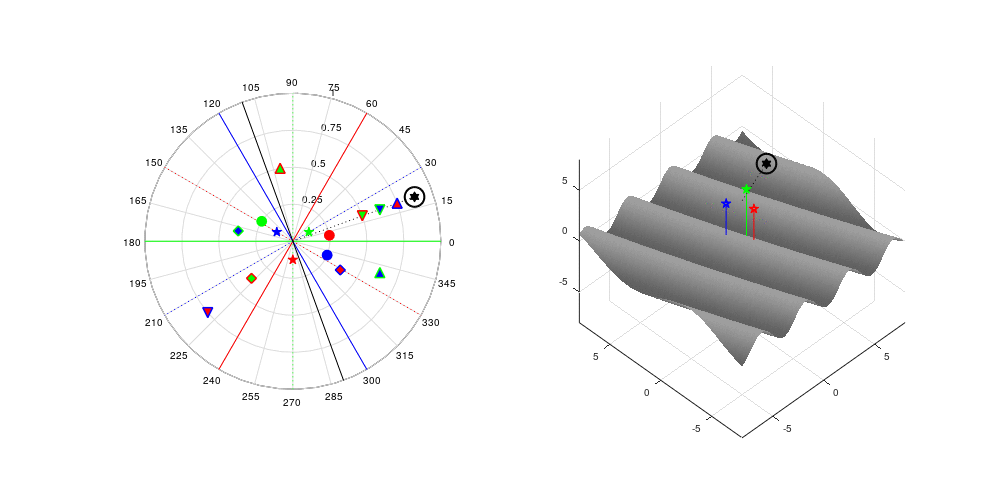
\includegraphics[width=0.9\textwidth]{../pictures/simul_POLY_3_R_50.png}
	\label{fig:example:simul_POLY_3_R_50}
	\caption*{Fonte: Autor.}
\end{figure}

\subsection{Função geral da simulção}

% Definir função base xyt e variáveis

Finalmente a função responsável por juntar todas as partes é \lstinline|w_xyt|, a base para a simulação, ela invoca as funções \lstinline|calc_AoA| e \lstinline|generate_fig| com os devidos parâmetros, além de garantir que os arquivos gerados sejam salvos corretamente.
Seus argumentos são, respectivamente, \lstinline|NOISE|, \lstinline|ATT|, \lstinline|CHG_PHI|, \lstinline|CHG_R|, \lstinline|CHG_THETA|, \lstinline|S_GIF|, \lstinline|S_DAT|, \lstinline|SNR|, \lstinline|range_step| e \lstinline|N_antenas|.

% \subsection{Outras funções}

% A função \lstinline|isoctave| confere se a corrente simulação está sendo realizada no GNU Octave, retornando um valor binário e não recebe qualquer parâmetro.
% O \autoref{cod:isoctave} apresenta uma versão simplificada da função \lstinline|isoctave| desenvolvida.

% \begin{lstfloat}[htbp]
% 	\centering
% 	\lstinputlisting[
% 			basicstyle=\ttfamily\small\setstretch{1},
% 			label=cod:isoctave,
% 			caption={Função \lstinline|isoctave|, simplificada.}
% 		]{../code/isoctave_alt.m}
% 	\caption*{Fonte: Autor.}
% \end{lstfloat}

% Falar sobre simular duas voltas na geometria


% Falar sobre exportação de arquivo .dat

